\documentclass[fleqn,12pt]{article}
\usepackage{amsmath}
\usepackage[colorlinks]{hyperref}
\usepackage{fullpage}
\setlength{\parindent}{0em}
\setlength{\parskip}{1em}
\usepackage{array}
\usepackage{tikz}
\usetikzlibrary{positioning}
\begin{document}
\thispagestyle{empty}

\section*{Logic pset 7}

Please answer \textbf{any three} of the following questions; each is
worth six points. Write your answers in your own words, making your
reasoning explicit. \textbf{Resource:} Chapter 8 of \textit{HLW}

\begin{enumerate}
\item Is there a valid proof with the following line fragments? Write
  your answer in the form of a short essay, using complete sentences.

  \begin{tabular}{>{\raggedleft\arraybackslash}p{1.5cm} >{\centering\arraybackslash}p{1.0cm} p{5cm} >{\raggedright\arraybackslash}p{3.5cm}}
    1 & (1) & $\exists x(Fx\to \forall yGy)$ & A \\
    \mbox{}  & \,\vdots & \\
    1 & (n) & $\exists xFx\to \forall yGy$ \end{tabular}

\item The sentence $P\to \exists xFx$ is not existential, and so is
  not a candidate for EE. But if there is a derivation of $\varphi$
  from $P\to Fa$ and auxiliary assumptions $\Delta$ that obeys the
  restrictions on EE (i.e.\ the name $a$ doesn't occur anywhere
  outside of the subproof), then is there also a derivation of
  $\varphi$ from $P\to \exists xFx$ and $\Delta$? Explain your answer.
  
\item Consider the two sentences $\forall xFx\to P$ and
  $\forall x(Fx\to P)$, where $x$ does not occur in $P$. Are these
  sentences logically equivalent? Justify your answer by providing
  proofs and/or models. Write out your answer clearly enough that it
  would convince somebody who doesn't already get it.

\item Consider the following two interpretations of the binary
  relation $R$, one with domain $\{ 1,2,3\}$ and the other with domain
  $\{ \alpha ,\beta ,\gamma \}$. Write a sentence that is true in one
  model but false in the other, and explain step by step how to
  determine its truth value in each. (Note that
  $1,2,3,\alpha ,\beta,\gamma$ are elements of the models; they are
  not names that can be used in your sentence.)

\begin{tabular}{cc}
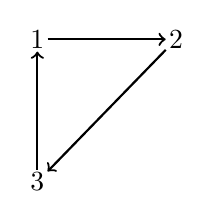
\begin{tikzpicture}[scale=1, every node/.style={inner sep=1pt, font=\normalsize}]
\node (a) {$1$};
\node[right=1.5cm of a] (b) {$2$};
\node[below=1.5cm of a] (c) {$3$};
\draw[->, thick] (a) -- (b);
\draw[->, thick] (b) -- (c);
\draw[->, thick] (c) -- (a);
\end{tikzpicture}

  &

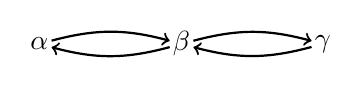
\begin{tikzpicture}[scale=1, every node/.style={inner sep=1pt, font=\normalsize}]
\node (a) {$\alpha$};
\node[right=1.5cm of a] (b) {$\beta$};
\node[right=1.5cm of b] (c) {$\gamma$};
% forward arrows
\draw[->, thick, bend left=15] (a) to (b);
\draw[->, thick, bend left=15] (b) to (c);
% backward arrows
\draw[->, thick, bend left=15] (b) to (a);
\draw[->, thick, bend left=15] (c) to (b);
\end{tikzpicture}    

\end{tabular}

\item For each of the following sentences, provide one interpretation
  in which it is true and another in which it is false. An
  interpretation may be presented by giving a set $M$ and a subset
  $R^M$ of $M\times M$, or it may be presented as an arrow diagram. In
  either case, explain step-by-step how to determine the truth value
  of the sentence in the model.
  
\begin{enumerate} \item $\forall x\forall y\exists z(Rxz\wedge Ryz)$
\item $\forall x(\exists yRyx\to \forall zRzx)$
  \end{enumerate}



\end{enumerate}



\end{document}


%%% Local Variables:
%%% mode: latex
%%% TeX-master: t
%%% End:
